\section{函数模板简介}
在重载 \lstinline@max@ 时,我们发现一个问题:如果我们只提供这两种重载:
\begin{lstlisting}
double max(double, double); //接收两个double类型参数
long long max(long long, long long); //接收两个long long类型参数
\end{lstlisting}
那么当我们调用 \lstinline@max(1,2)@ 时就会出现二义性问题。这是因为,\lstinline@int@ 隐式类型转换为 \lstinline@double@ 类型或 \lstinline@long long@ 的优先性相同,编译器就会面临两难处境,不知该转换成哪种类型是好。解决的方法也很简单,我们再重载一个 \lstinline@int max(int,int)@ 就好了嘛。
\begin{lstlisting}
int max(int, int); //接收两个int类型参数
\end{lstlisting}\par
但这不是一劳永逸的方案。如果我们之后又需要做两个 \lstinline@long double@ 求最大值的操作,那么我们还需要再作如下重载:
\begin{lstlisting}
long double max(long double, long double); //接收两个long double类型参数
\end{lstlisting}\par
实际操作中我们不一定碰到这么多类型一起出现的情况,但是为了同样的功能写这么多重载,而且每次用别的类型时都要考虑``是否还要加一个重载'',这是很麻烦的。能不能有一种方案,可以针对各种不同的类型,一次性给出同样的解决方案呢?\textbf{泛型编程(Generic programming)}的理念就这样应运而生了。\par
泛型编程理念的核心在于,我们无需考虑具体的数据类型,只要给它们一套通用的\textbf{模板(Template)}即可。而编译器会根据代码中的需要,生成对应的函数\textbf{实例(Instance)}。\par
以求两数最大值的函数为例,我们可以定义如下的函数模板(Function template)。
\begin{lstlisting}
template<typename T> //假设一个模板参数T,T可以是任何一种类型
T maximum(T a, T b) { //返回类型为T,接收两个T类型的参数
    return a > b ? a : b; //用条件表达式实现,代码更简洁
}
\end{lstlisting}
这里之所以使用 \lstinline@maxinum@ 名字是因为 \lstinline@std@ 命名空间中已有 \lstinline@max@ 模板,为了防止重名引起一系列麻烦,就在此处换用它名。\footnote{我们会在第七章中讲解如何规避这类问题。}\par
这里我们用 \lstinline@template@ 关键字定义一个模板,这个模板有一个模板参数,名为 \lstinline@T@,它就是``某个类型''。\par
然后是函数定义(声明)部分,我们指定了这个函数模板的返回类型为 \lstinline@T@,名称为 \lstinline@maximum@,接收两个 \lstinline@T@ 类型参数。\par
再看函数体,这里涉及到了一个条件表达式,用到了条件运算符``@? :@''。条件运算符的功能很容易理解,它接收三个操作数,如果第一个操作数的值是 \lstinline@true@\footnote{如果第一操作数不是 \lstinline@bool@ 类型,会进行布尔转换变为 \lstinline@bool@ 类型,下同。},那么条件运算符的返回值就是第二操作数;如果第一个操作数的值是 \lstinline@false@,那么条件运算符的返回值就是第三操作数。在本函数模板中就可以这样理解:如果 \lstinline@a>b@ 得到 \lstinline@true@,就返回 \lstinline@a@;否则返回 \lstinline@b@——这和使用 \lstinline@if@-\lstinline@else@ 结构的作用是相似的。\par
接下来我们就可以在主函数中使用 \lstinline@maximum@ 函数模板了。非常简单:
\begin{lstlisting}
int main() {
    cout << maximum(1, 2) << endl; //调用int maximum(int,int)
    cout << maximum(1ll, 0ll) << endl;
    //调用long long maximum(long long,long long)
    cout << maximum(1., 2.) << endl; //调用double maximum(double,double)
    cout << maximum(1.l, .1l) << endl;
    //调用long double maximum(long double,long double)
}
\end{lstlisting}
编译器在知道了这个函数模板之后,每当遇到需要的函数(比如,调用 \lstinline@maximum(1,2)@,需要一个 \lstinline@maximum(int,int)@),就会根据这个模板,制造一个 \lstinline@maximum(int,int)@ 函数来匹配它。\par
那么在这个主函数中我们用四种类型的参数调用 \lstinline@maximum@ 函数,编译器就会根据需要,制造四个函数:
\begin{lstlisting}
int max(int a, int b) { //int版本
    return a > b ? a : b;
}
long long max(long long a, long long b) { //long long版本
    return a > b ? a : b;
}
double max(double a, double b) { //double版本
    return a > b ? a : b;
}
long double max(long double a, long double b) { //long double版本
    return a > b ? a : b;
}
\end{lstlisting}\par
所以说,使用函数模板相当于我们给编译器提供了一个范本,而编译器会根据这个范本来制造对应类型的重载。这样不用我们手动写一大堆函数重载了。\par
\begin{figure}[htbp]
    \centering
    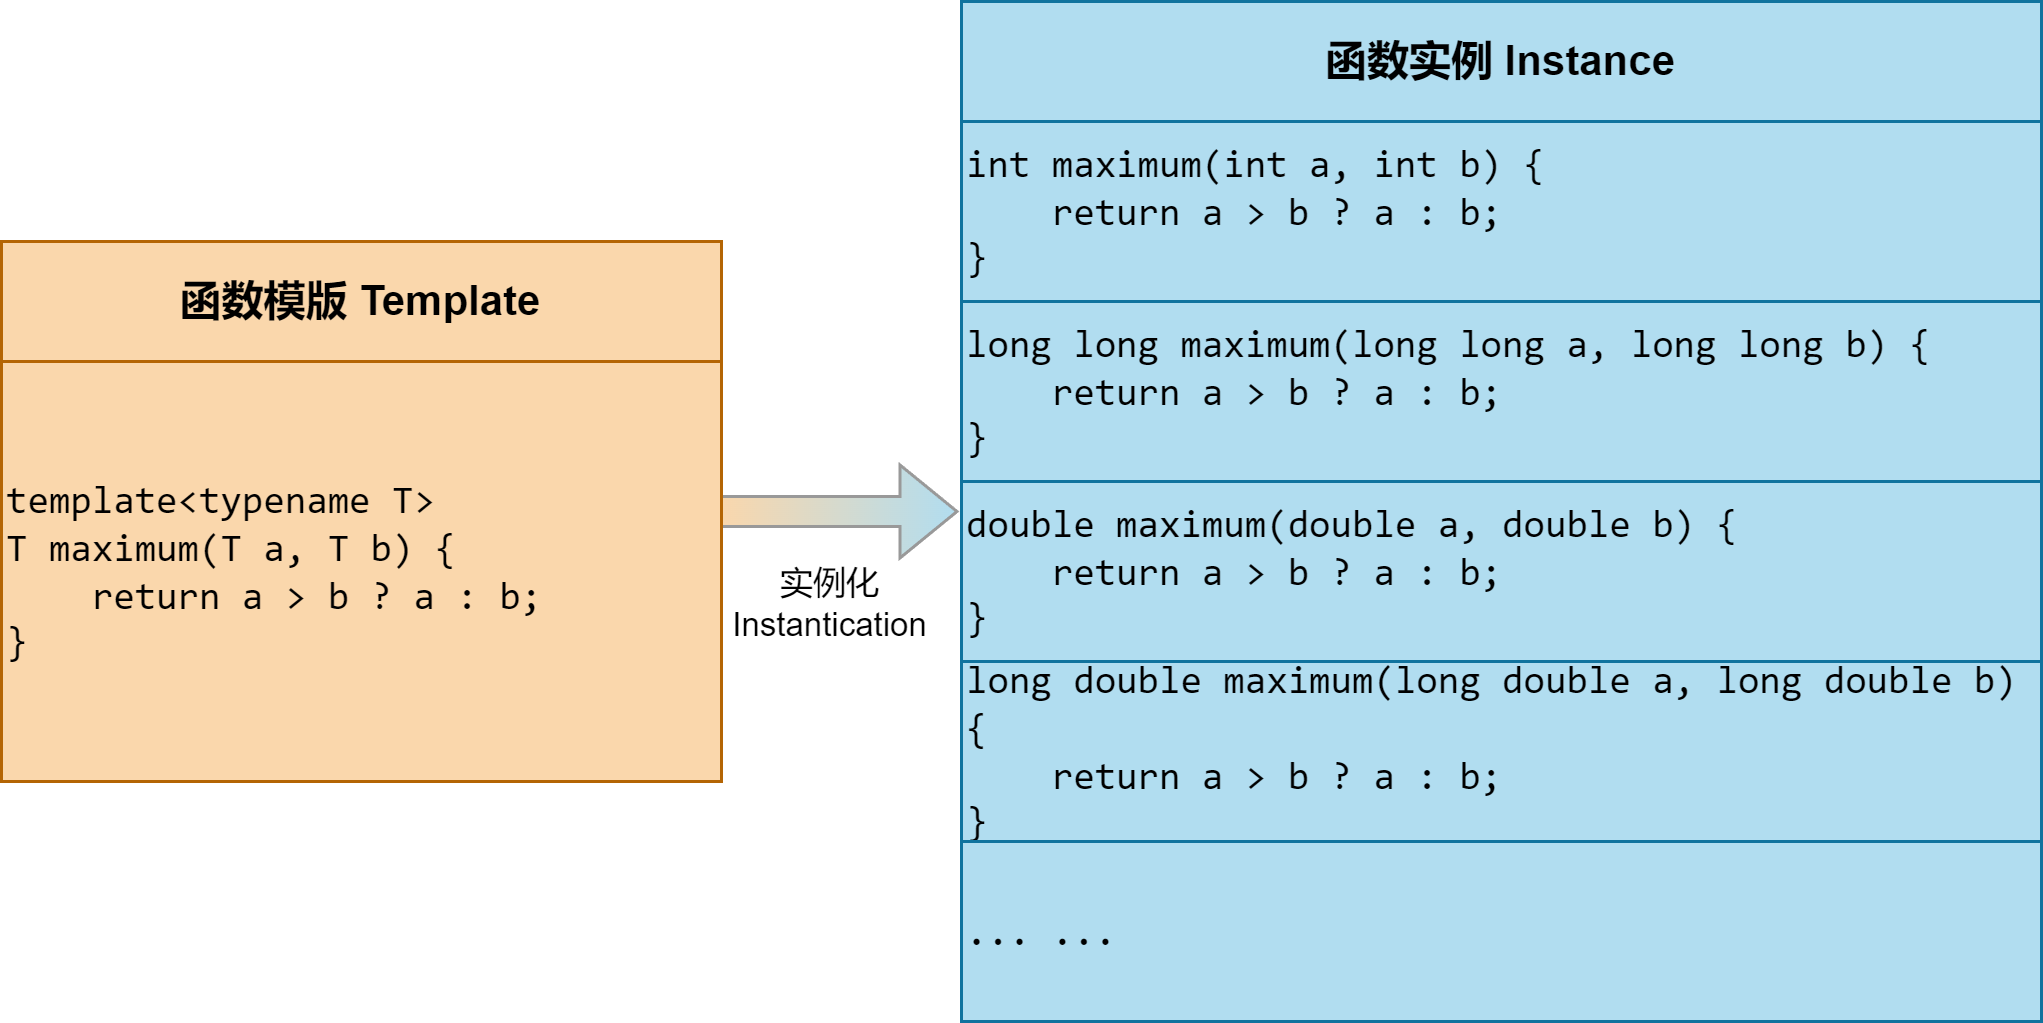
\includegraphics[width=0.9\textwidth]{.//images/generalized_parts/04_function_template_and_instance.drawio.png}
    \caption{从函数模板到函数实例}
\end{figure}
我们可以再加一个三数求最值的函数模板。这也是一种函数重载。
\begin{lstlisting}
template<typename T> //假设一个模板参数T,T可以是任何一种类型
T maximum(T a, T b) { //返回类型为T,接收两个T类型的参数
    return a > b ? a : b; //用条件表达式实现,代码更简洁
}
template<typename T> //注意,每次声明(定义)模板都需要写template,不能共用
T maximum(T a, T b, T c) { //返回类型为T,接收三个T类型的参数
    return a > b ? (a > c ? a : c) : (b > c ? b : c); //请读者自行分析
}
\end{lstlisting}
本节只是对模板函数和泛型编程作一个简单介绍,我们会在第十一章更详细地探讨这方面的问题。\par
